\documentclass[a4paper, 12pt]{article}

\usepackage{mathtext}
\usepackage[T2A]{fontenc}
\usepackage[utf8]{inputenc}
\usepackage[russian]{babel}

\usepackage{amsmath}
\usepackage{titlesec}
\usepackage{scrextend}
\usepackage{graphicx}
\usepackage{tikz}
\usetikzlibrary{shapes.misc}
\usepackage{pdflscape}

\DeclareSymbolFont{T2Aletters}{T2A}{cmr}{m}{it}
\graphicspath{ {./images/} }

% Установки для отрисовки решеток кодера
\tikzstyle{lightedge}=[dashed]
\tikzstyle{mainedge}=[solid]
\tikzstyle{activeedge}=[green, very thick]
\tikzstyle{inputBit}=[rectangle,fill=red, text=white]
\tikzstyle{outputBit}=[rectangle,fill=blue, text=white]
\tikzstyle{pointer}=[orange,->,dashed]

\newcounter{ctra}
\newcommand{\trellisEdges}[2]{
  \setcounter{ctra}{#2}
  \pgfmathtruncatemacro{\xplusone}{#1 + 1}
  \ifodd\value{ctra}
      \draw[mainedge] (s#1#2) -- (s\xplusone2);
  \else
      \draw[mainedge] (s#1#2) -- (s\xplusone0);
  \fi
  \ifodd\value{ctra}
      \draw[lightedge] (s#1#2) -- (s\xplusone3);
  \else
      \draw[lightedge] (s#1#2) -- (s\xplusone1);
  \fi
}

% #1=x; #2=y; #3=In; #4=Out
\newcommand{\trellisInOut}[4]{
  \node[inputBit] (in#1) at (#1+0.5,4) {#3};
  \node[outputBit] (out#1) at (#1+0.5,5) {#4};
  \draw[pointer] (in#1) -- (#1+0.5,#2);
}

% #1=x; #2=y; #3=In
\newcommand{\trellisIn}[2]{
  \node[outputBit] (in#1) at (#1+0.5,4) {#2};
}


\author{Анатолий Копыл}
\title{Курсовая работа}

\begin{document}

\section{Исходные данные}
\[ m=41 \]
\begin{center}
  \begin{tabular}{ | p{5cm} | p{5cm} | p{5cm} | } 
    \hline
    Предельные уровни аналогового сигнала \(a_{min}\), \(a_{max}\) (В) & \(a_{max}=25,6\) В;\newline\(a_{min}=-25,6\) В & Внести свои данные \\
    \hline
    Верхняя частота спектра аналогового сигнала \(f_В\) & \(f_В =(1+m\cdot 10^{-2})\cdot 10^4\) & \(f_В =14100\) \\ 
    \hline
    Заданный уровень квантования & \(j=500-3\cdot m\) & 377 \\
    \hline
    Спектральная плотность мощности флуктуационной помехи & 41 & \(N_0=2,3\cdot 10^{-7}\, В^2/Гц\)\\
    \hline
    q - номер тактового интервала ошибки & \(q=m\mod{3}+1\) & \(q=3\)\\
    \hline
    Вид модуляции & КАМ-16 & \\
    \hline
  \end{tabular}
\end{center}

\section{Аналого-цифровой преобразователь}
\[ \Delta t \leq \frac{1}{2f_B}=\frac1 {2\cdot 14100} = 3,546\cdot 10^{-5}\, с \]
\[ f_d=\frac{1}{\Delta t}\geq 2f_B=\frac{1}{3,546\cdot 10^{-5}}=28200 \]
\[ 377_{10}=101111001_2 \]
\[ k=9;\, L=2^9 = 512 \]

\section{Кодер}
\begin{center}
  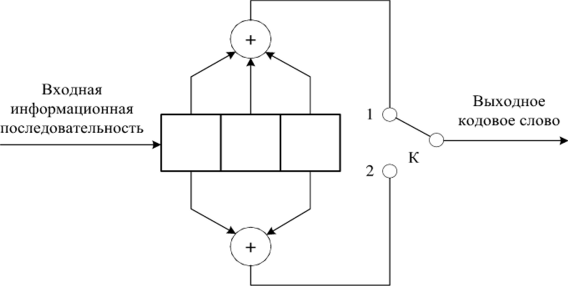
\includegraphics[scale=0.8]{coder}

  \begin{tabular}{ | c | c | c | c | c | c | c | c | c | c | }
    \hline
    Входной сигнал &1&0&1&1&1&1&0&0&1\\
    \hline
    Выходной сигнал &11&10&00&01&10&10&01&11&11\\
    \hline
  \end{tabular}
\end{center}

\subsection{Решетка кодера}

\begin{tikzpicture}[x=1.2cm, y=-1cm]
  \node at (-0.5,0) [left] {$s_1=00$};
  \node at (-0.5,1) [left] {$s_2=10$};
  \node at (-0.5,2) [left] {$s_3=01$};
  \node at (-0.5,3) [left] {$s_4=11$};

  % Nodes
  \foreach \x in {0,...,9} {
    \node at (\x,-.7) {$\x$};
    \foreach \y in {0,...,3} {
      \node (s\x\y) at (\x,\y) [circle,fill=black,scale=0.7] {};
    }
  }

  % Edges
  \trellisEdges{0}{0}
  \trellisEdges{1}{0}
  \trellisEdges{1}{1}
  \foreach \x in {2,...,8} {
    \foreach \y in {0,...,3} {
      \trellisEdges{\x}{\y}
    }
  }

  % Inputs and Outputs
  \node at (-0.5,4) [left] {Входной бит};
  \node at (-0.5,5) [left] {Результат};

  \trellisInOut{0}{0.5}{1}{11}
  \trellisInOut{1}{1.5}{0}{10}
  \trellisInOut{2}{1.5}{1}{00}
  \trellisInOut{3}{2}{1}{01}
  \trellisInOut{4}{3}{1}{10}
  \trellisInOut{5}{3}{1}{10}
  \trellisInOut{6}{2.5}{0}{01}
  \trellisInOut{7}{1}{0}{11}
  \trellisInOut{8}{0.5}{1}{11}
\end{tikzpicture}

Длительность двоичного символа \(T_В\) на выходе кодера:
\[T_В=\frac{\Delta t}{2k}=\frac{3,546\cdot 10^{-5}}{2\cdot 9}=
1,97\cdot 10^{-6}\,с\]

\section{Декодер}
По каналу передавался код \(\overline{u}=11 10 00 01 10 10 01 11 11\).
Ошибка произошла на тактовом интервале \(q=3\).
Таким образом, на вход декодера поступает последовательность 
\(\overline{Z}=11 \dot{0}0 00 01 10 10 01 11 11\). Точкой обозначен ошибочно принятый символ.

\subsection{Диаграмма декодера}

\begin{tikzpicture}[x=1.2cm, y=-1cm,  
  highlight/.style={circle,fill=blue,text=white,scale=0.7}
  ]

  \node at (-0.5,0) [left] {$s_1=00$};
  \node at (-0.5,1) [left] {$s_2=10$};
  \node at (-0.5,2) [left] {$s_3=01$};
  \node at (-0.5,3) [left] {$s_4=11$};

  % Nodes
  \foreach \x in {0,...,9} {
    \node at (\x,-.7) {$\x$};
    \foreach \y in {0,...,3} {
      \node (s\x\y) at (\x,\y) [circle,fill=black,scale=0.7] {};
    }
  }

  \node at (0,0) [highlight] {};
  \node at (1,0) [highlight,label=left:{$2$}] {};
  \node at (1,1) [highlight,label=left:{$0$}] {};

  \node at (2,0) [highlight,label=left:{$0$}] {};
  \node at (2,1) [highlight,label=left:{$2$}] {};
  \node at (2,2) [highlight,label=left:{$1$}] {};
  \node at (2,3) [highlight,label=left:{$1$}] {};

  \node at (3,0) [highlight,label=left:{$\frac{0}{2}$}] {};
  \node at (3,1) [highlight,label=left:{$\frac{2}{0}$}] {};
  \node at (3,2) [highlight,label=left:{$\frac{1}{1}$}] {};
  \node at (3,3) [highlight,label=left:{$\frac{1}{1}$}] {};

  \node at (4,0) [highlight,label=left:{$\frac{1}{1}$}] {};
  \node at (4,1) [highlight,label=left:{$\frac{1}{1}$}] {};
  \node at (4,2) [highlight,label=left:{$\frac{2}{0}$}] {};
  \node at (4,3) [highlight,label=left:{$\frac{0}{2}$}] {};

  \node at (5,0) [highlight,label=left:{$\frac{1}{1}$}] {};
  \node at (5,1) [highlight,label=left:{$\frac{1}{1}$}] {};
  \node at (5,2) [highlight,label=left:{$\frac{0}{2}$}] {};
  \node at (5,3) [highlight,label=left:{$\frac{2}{0}$}] {};

  \node at (6,0) [highlight,label=left:{$\frac{1}{1}$}] {};
  \node at (6,1) [highlight,label=left:{$\frac{1}{1}$}] {};
  \node at (6,2) [highlight,label=left:{$\frac{0}{2}$}] {};
  \node at (6,3) [highlight,label=left:{$\frac{2}{0}$}] {};

  \node at (7,0) [highlight,label=left:{$\frac{1}{1}$}] {};
  \node at (7,1) [highlight,label=left:{$\frac{1}{1}$}] {};
  \node at (7,2) [highlight,label=left:{$\frac{2}{0}$}] {};
  \node at (7,3) [highlight,label=left:{$\frac{0}{2}$}] {};

  \node at (8,0) [highlight,label=left:{$\frac{2}{0}$}] {};
  \node at (8,1) [highlight,label=left:{$\frac{0}{2}$}] {};
  \node at (8,2) [highlight,label=left:{$\frac{1}{1}$}] {};
  \node at (8,3) [highlight,label=left:{$\frac{1}{1}$}] {};

  \node at (9,0) [highlight,label=left:{$\frac{2}{0}$}] {};
  \node at (9,1) [highlight,label=left:{$\frac{0}{2}$}] {};
  \node at (9,2) [highlight,label=left:{$\frac{1}{1}$}] {};
  \node at (9,3) [highlight,label=left:{$\frac{1}{1}$}] {};

  % Edges
  \trellisEdges{0}{0}
  \trellisEdges{1}{0}
  \trellisEdges{1}{1}
  \foreach \x in {2,...,8} {
    \foreach \y in {0,...,3} {
      \trellisEdges{\x}{\y}
    }
  }

  % Inputs
  \node at (-0.5,4) [left] {Входная пара};

  \trellisIn{0}{11}
  \trellisIn{1}{00}
  \trellisIn{2}{00}
  \trellisIn{3}{01}
  \trellisIn{4}{10}
  \trellisIn{5}{10}
  \trellisIn{6}{01}
  \trellisIn{7}{11}
  \trellisIn{8}{11}
\end{tikzpicture}

\begin{tikzpicture}[x=1.2cm, y=-1cm,  
  highlight/.style={circle,fill=blue,text=white,scale=0.7}
  ]

  \node at (-0.5,0) [left] {$s_1=00$};
  \node at (-0.5,1) [left] {$s_2=10$};
  \node at (-0.5,2) [left] {$s_3=01$};
  \node at (-0.5,3) [left] {$s_4=11$};

  % Edges
  \trellisEdges{0}{0}
  \trellisEdges{1}{0}
  \trellisEdges{1}{1}
  \foreach \x in {2,...,8} {
    \foreach \y in {0,...,3} {
      \trellisEdges{\x}{\y}
    }
  }

  % Nodes
  \foreach \x in {0,...,9} {
    \node at (\x,-.7) {$\x$};
    \foreach \y in {0,...,3} {
      \node (s\x\y) at (\x,\y) [circle,fill=black,scale=0.7] {};
    }
  }

  \node at (0,0) [highlight] {};
  \node at (1,0) [highlight,label=left:{$2$}] {};
  \node at (1,1) [highlight,label=left:{$0$}] {};

  \node at (2,0) [highlight,label=left:{$0$}] {};
  \node at (2,1) [highlight,label=left:{$2$}] {};
  \node at (2,2) [highlight,label=left:{$1$}] {};
  \node at (2,3) [highlight,label=left:{$1$}] {};

  \node at (3,0) [highlight,label=left:{$\frac{0}{2}$}] {$\frac23$};
  \node at (3,1) [highlight,label=left:{$\frac{2}{0}$}] {$\frac41$};
  \node at (3,2) [highlight,label=left:{$\frac{1}{1}$}] {$\frac52$};
  \node at (3,3) [highlight,label=left:{$\frac{1}{1}$}] {$\frac52$};

  \node at (2.5,1) [text=red] {$\times$};
  \node at (2.5,0.5) [text=red] {$\times$};
  \node at (2.5,1.5) [text=red] {$\times$};
  \node at (2.5,2) [text=red] {$\times$};
  \node at (1.5,0.5) [text=red] {$\times$};

  \draw[activeedge] (s00) -- (s10);
  \draw[activeedge] (s00) -- (s11);
  \draw[activeedge] (s10) -- (s20);
  \draw[activeedge] (s11) -- (s22);
  \draw[activeedge] (s20) -- (s30);
  \draw[activeedge] (s22) -- (s31);
  \draw[activeedge] (s11) -- (s23);
  \draw[activeedge] (s23) -- (s32);
  \draw[activeedge] (s23) -- (s33);

  \node at (4,0) [highlight,label=left:{$\frac{1}{1}$}] {};
  \node at (4,1) [highlight,label=left:{$\frac{1}{1}$}] {};
  \node at (4,2) [highlight,label=left:{$\frac{2}{0}$}] {};
  \node at (4,3) [highlight,label=left:{$\frac{0}{2}$}] {};

  \node at (5,0) [highlight,label=left:{$\frac{1}{1}$}] {};
  \node at (5,1) [highlight,label=left:{$\frac{1}{1}$}] {};
  \node at (5,2) [highlight,label=left:{$\frac{0}{2}$}] {};
  \node at (5,3) [highlight,label=left:{$\frac{2}{0}$}] {};

  \node at (6,0) [highlight,label=left:{$\frac{1}{1}$}] {};
  \node at (6,1) [highlight,label=left:{$\frac{1}{1}$}] {};
  \node at (6,2) [highlight,label=left:{$\frac{0}{2}$}] {};
  \node at (6,3) [highlight,label=left:{$\frac{2}{0}$}] {};

  \node at (7,0) [highlight,label=left:{$\frac{1}{1}$}] {};
  \node at (7,1) [highlight,label=left:{$\frac{1}{1}$}] {};
  \node at (7,2) [highlight,label=left:{$\frac{2}{0}$}] {};
  \node at (7,3) [highlight,label=left:{$\frac{0}{2}$}] {};

  \node at (8,0) [highlight,label=left:{$\frac{2}{0}$}] {};
  \node at (8,1) [highlight,label=left:{$\frac{0}{2}$}] {};
  \node at (8,2) [highlight,label=left:{$\frac{1}{1}$}] {};
  \node at (8,3) [highlight,label=left:{$\frac{1}{1}$}] {};

  \node at (9,0) [highlight,label=left:{$\frac{2}{0}$}] {};
  \node at (9,1) [highlight,label=left:{$\frac{0}{2}$}] {};
  \node at (9,2) [highlight,label=left:{$\frac{1}{1}$}] {};
  \node at (9,3) [highlight,label=left:{$\frac{1}{1}$}] {};

  % Inputs and Outputs
  \node at (-0.5,4) [left] {Входная пара};

  \trellisIn{0}{11}
  \trellisIn{1}{00}
  \trellisIn{2}{00}
  \trellisIn{3}{01}
  \trellisIn{4}{10}
  \trellisIn{5}{10}
  \trellisIn{6}{01}
  \trellisIn{7}{11}
  \trellisIn{8}{11}
\end{tikzpicture}

\end{document}
